% Options for packages loaded elsewhere
\PassOptionsToPackage{unicode}{hyperref}
\PassOptionsToPackage{hyphens}{url}
%
\documentclass[
]{article}
\usepackage{amsmath,amssymb}
\usepackage{lmodern}
\usepackage{iftex}
\ifPDFTeX
  \usepackage[T1]{fontenc}
  \usepackage[utf8]{inputenc}
  \usepackage{textcomp} % provide euro and other symbols
\else % if luatex or xetex
  \usepackage{unicode-math}
  \defaultfontfeatures{Scale=MatchLowercase}
  \defaultfontfeatures[\rmfamily]{Ligatures=TeX,Scale=1}
\fi
% Use upquote if available, for straight quotes in verbatim environments
\IfFileExists{upquote.sty}{\usepackage{upquote}}{}
\IfFileExists{microtype.sty}{% use microtype if available
  \usepackage[]{microtype}
  \UseMicrotypeSet[protrusion]{basicmath} % disable protrusion for tt fonts
}{}
\makeatletter
\@ifundefined{KOMAClassName}{% if non-KOMA class
  \IfFileExists{parskip.sty}{%
    \usepackage{parskip}
  }{% else
    \setlength{\parindent}{0pt}
    \setlength{\parskip}{6pt plus 2pt minus 1pt}}
}{% if KOMA class
  \KOMAoptions{parskip=half}}
\makeatother
\usepackage{xcolor}
\usepackage[margin=1in]{geometry}
\usepackage{longtable,booktabs,array}
\usepackage{calc} % for calculating minipage widths
% Correct order of tables after \paragraph or \subparagraph
\usepackage{etoolbox}
\makeatletter
\patchcmd\longtable{\par}{\if@noskipsec\mbox{}\fi\par}{}{}
\makeatother
% Allow footnotes in longtable head/foot
\IfFileExists{footnotehyper.sty}{\usepackage{footnotehyper}}{\usepackage{footnote}}
\makesavenoteenv{longtable}
\usepackage{graphicx}
\makeatletter
\def\maxwidth{\ifdim\Gin@nat@width>\linewidth\linewidth\else\Gin@nat@width\fi}
\def\maxheight{\ifdim\Gin@nat@height>\textheight\textheight\else\Gin@nat@height\fi}
\makeatother
% Scale images if necessary, so that they will not overflow the page
% margins by default, and it is still possible to overwrite the defaults
% using explicit options in \includegraphics[width, height, ...]{}
\setkeys{Gin}{width=\maxwidth,height=\maxheight,keepaspectratio}
% Set default figure placement to htbp
\makeatletter
\def\fps@figure{htbp}
\makeatother
\setlength{\emergencystretch}{3em} % prevent overfull lines
\providecommand{\tightlist}{%
  \setlength{\itemsep}{0pt}\setlength{\parskip}{0pt}}
\setcounter{secnumdepth}{5}
\usepackage{setspace}
\doublespacing
\usepackage{booktabs}
\usepackage{longtable}
\usepackage{array}
\usepackage{multirow}
\usepackage{wrapfig}
\usepackage{float}
\usepackage{colortbl}
\usepackage{pdflscape}
\usepackage{tabu}
\usepackage{threeparttable}
\usepackage{threeparttablex}
\usepackage[normalem]{ulem}
\usepackage{makecell}
\usepackage{xcolor}
\ifLuaTeX
  \usepackage{selnolig}  % disable illegal ligatures
\fi
\usepackage[]{natbib}
\bibliographystyle{plainnat}
\IfFileExists{bookmark.sty}{\usepackage{bookmark}}{\usepackage{hyperref}}
\IfFileExists{xurl.sty}{\usepackage{xurl}}{} % add URL line breaks if available
\urlstyle{same} % disable monospaced font for URLs
\hypersetup{
  pdftitle={Assignment 1 Routine Care},
  pdfauthor={Martijn Koster, 6234119; Jurrian van de Kraats, 5961688; Tim Poorthuis, 0651478},
  hidelinks,
  pdfcreator={LaTeX via pandoc}}

\title{Assignment 1 Routine Care}
\author{Martijn Koster, 6234119 \and Jurrian van de Kraats, 5961688 \and Tim Poorthuis, 0651478}
\date{2023-02-15}

\begin{document}
\maketitle

\newpage

\hypertarget{introduction}{%
\section{Introduction}\label{introduction}}

In this paper we will examine whether there is a causal effect from elderly people who have received an influenza vaccine and the likelihood of hospitalization. This will be examined by using the patient records dataset and different modeling methods using propensity scores, to account for confounders.

\hypertarget{methods}{%
\section{Methods}\label{methods}}

\hypertarget{examening-the-causal-structure}{%
\subsection{Examening the causal structure}\label{examening-the-causal-structure}}

Domain knowledge was used to create a DAG (Figure \ref{fig:dag} ) that explains the causal structure present in the data. The variable `contact with chiropractor (GP)' forms a proxy for the unobserved variable healthy lifestyle. Getting the influenza vaccine is connected to age and contact with GP. Having obtained a influenza vaccination was associated with a lower risk for adverse cardiovascular events \citep{behrouzi}. Having pulmonary disease and diabetes increases the chance for cardiovascular disease \citep{nhg}. Sex forms a confounder between hospitalization and healthy lifestyle \citep{loef} which in turn causes the afore mentioned diseases.\\
The causal paths of the DAG should be examined to asses whether unbiased causal inference is possible. There is a flow of statistical information through open backdoor paths due to observed and unobserved confounders. The eventual model would need to adjust for these confounders in order to perform an unbiased causal inference.

\begin{figure}
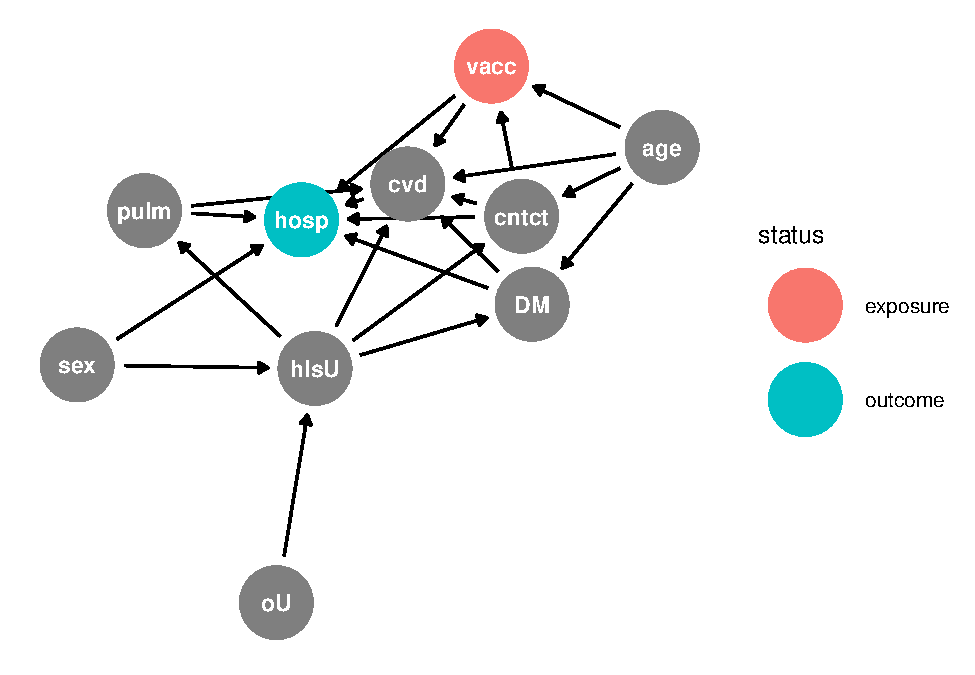
\includegraphics[width=0.5\linewidth]{Assignment_files/figure-latex/dag-1} \caption{DAG model with Vaccine as exposure and hospitalization as outcome}\label{fig:dag}
\end{figure}

\hypertarget{statistical-methods}{%
\subsection{Statistical Methods}\label{statistical-methods}}

\hypertarget{baseline-characteristics}{%
\subsubsection{Baseline Characteristics}\label{baseline-characteristics}}

The electronic patient records dataset consist of eight variables. The variables age and contact with a chiropractor were continues, the variables vaccination status, sex, cardiovascular disease, pulmonary disease, diabetes and hospitalization were binominal. Table \ref{tab:des} presents the baseline characteristics of 40000 individuals who were included in the study.\\
\hspace*{0.333em}\hspace*{0.333em}Baseline characteristics stratified by the study outcome indicate that 254 of the respondents were hospitalized. Respondents who were hospitalized were older (79.68 vs 75.63), had more contact with the GP (21.08 vs 14.71), were less often female (48.43\%), had more often cardiovascular disease (72.05\% vs 49.25\%) and more often Diabetes (11.42\% vs 6.51\%).

\begin{table}[!h]

\caption{\label{tab:des}Baseline Characteristics stratified by Influenza vaccination received and Hospitalisation}
\centering
\begin{tabular}[t]{llllll}
\toprule
\multicolumn{1}{c}{ } & \multicolumn{1}{c}{ } & \multicolumn{2}{c}{Influenza vaccination received} & \multicolumn{2}{c}{Hospitalized} \\
\cmidrule(l{3pt}r{3pt}){3-4} \cmidrule(l{3pt}r{3pt}){5-6}
Characteristics & Total & Yes & No & Yes & No\\
\midrule
N & 40000 & 29616 & 10384 & 254 & 39746\\
Age, mean (SD) & 75.65 (6.97) & 75.9 (6.83) & 74.97 (7.32) & 79.68 (7.2) & 75.63 (6.97)\\
Contact, mean (SD) & 14.75 (11.54) & 15.85 (11.73) & 11.64 (10.38) & 21.08 (15.59) & 14.71 (11.5)\\
Female, n (\%) & 24763 (61.91) & 18022 (60.85) & 6741 (64.92) & 123 (48.43) & 24640 (61.99)\\
Pulmonary disease, n (\%) & 4937 (12.34) & 4244 (14.33) & 693 (6.67) & 60 (14.33) & 4877 (12.27)\\
\addlinespace
Cardiovascular disease, n (\%) & 19757 (49.39) & 15702 (53.02) & 4055 (39.05) & 183 (72.05) & 19574 (49.25)\\
Diabetes mellitus, n(\%) & 2618 (6.54) & 2223 (7.51) & 395 (3.8) & 29 (11.42) & 2589 (6.51)\\
Received Influenza Vaccination, n (\%) &  &  &  & 184 (72.44) & 29432 (74.05)\\
\bottomrule
\end{tabular}
\end{table}

\hypertarget{propensity-scores-ps}{%
\subsubsection{Propensity Scores (PS)}\label{propensity-scores-ps}}

In order to control for confounding, a PS was estimated by fitting a logistic regression. A PS gives the probability being vaccinated for the respondents. Based on the DAG (Figure \ref{fig:dag} ) the variables: age, sex, cardiovascular disease, pulmonary disease, diabetis mellitus, and GP contact were used in the PS model. For the variables age and contact a spline is used \citep{Tian}.\\
\hspace*{0.333em}\hspace*{0.333em}\hspace*{0.333em}\hspace*{0.333em}In Figure \ref{fig:psscore}, the PS for vaccinated and unvaccinated individuals appear to be well-balanced, supporting the positivity assumption, which means that both treatement groups have a chance to get the treatment given the covariates \citep{westreich}.

\hypertarget{ps-as-covariate}{%
\subsubsection{PS as Covariate}\label{ps-as-covariate}}

The first adjusted model is to use the PS as a covariate. In a observational study the treated and untreated group have an equal distribution given that these are divided in groups of a constant propensity. The propensity score can be used as a baseline variable to account for the dimensional difference between groups since it is assumed that the treatment is unconfounded given this propensity score \citep{schafer}.

\hypertarget{inverse-probability-weighting-ipw}{%
\subsubsection{Inverse Probability Weighting (IPW)}\label{inverse-probability-weighting-ipw}}

With the aforementioned propensity scores, IPW is calculated by \(\frac{1}{PS}\) for the vaccinated group and \(\frac{1}{1-PS}\) for the unvaccinated. IPW creates a pseudo-population by equaling the effect of the confounders mimicking a random control trial. \citep{shiba}.

Two models were created, one with stabilized- and one with unstabilized weights. When using stabilized weights the numerator model also includes confounders, giving more stable estimates compared to the unstabilized weights \citep{ipw}. In both models bootstrapping was used to account for the inflated sample size of the pseudo population.

\begin{figure}
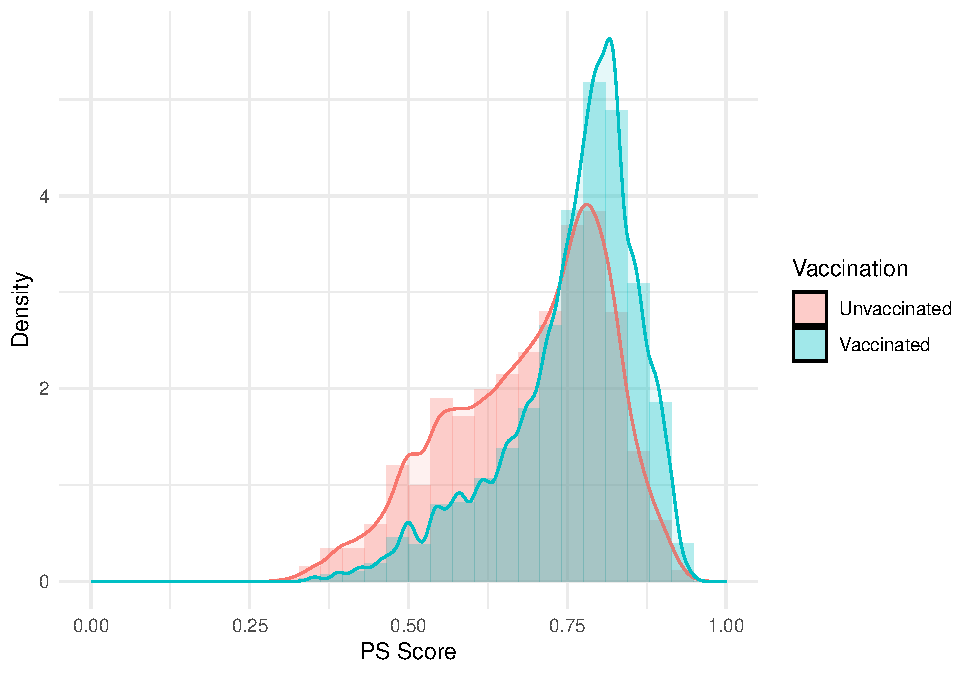
\includegraphics[width=0.7\linewidth]{Assignment_files/figure-latex/psscore-1} \caption{Distribution of the Propensity score for participants who received a vaccination compared with those who did not receive a vaccination}\label{fig:psscore}
\end{figure}

\hypertarget{results}{%
\section{Results}\label{results}}

Table \ref{tab:res} shows the crude association between vaccination status and hospitalization was examined using logistic regression, and the odds ratio was found to be 0.921 (95\% CI: 0.699, 1.214), indicating a non-significant association (p = 0.562). The C-statistic, a measure of discrimination, was 0.508, suggesting poor predictive performance of the model.\\
\hspace*{0.333em}\hspace*{0.333em}\hspace*{0.333em}\hspace*{0.333em}Considering the second model in Table \ref{tab:res}, which presents the PS as covariate, the odds ratio suggests a significant negative association (adjusted OR: 0.635. 95\% CI 0.478 to 0.843; p \textless.001). The C-Statistic of 0.679 suggests that the model has moderate discriminatory power.\\
\hspace*{0.333em}\hspace*{0.333em}\hspace*{0.333em}\hspace*{0.333em}The IPW model with unstabilised weights yields significant negative association between the exposure and outcome variable (adjusted OR: 0.617, 95\%CI 0.523 to 0.728; p \textless.001). The model presents moderate discriminatory power, where C = 0.573.\\
\hspace*{0.333em}\hspace*{0.333em}\hspace*{0.333em}\hspace*{0.333em}The last model in Table \ref{tab:res} is an IPW model with stabilised weights. This model also presents a negative association between vaccination and hospitalisation (Adjusted OR: 0.617, 95\% CI 0.509 to 0.748; p \textless.001). The C-statistic suggests moderate discriminatory power (C= 0.573).

\begin{table}[!h]

\caption{\label{tab:res}Association between influenza vaccination and hospitalization (n=40000)}
\centering
\begin{tabular}[t]{lllr}
\toprule
Model Specification & OR (95\% CI) & P-Value & C-Statistic\\
\midrule
Unadjusted & 0.921 (0.699 to 1.214) & 0.562 & 0.508\\
PS as covariate & 0.635 (0.478 to 0.843) & <.001 & 0.679\\
Unstabilised IPW & 0.617 (0.523 to 0.728) & <.001 & 0.573\\
Stabilised IPW & 0.617 (0.509 to 0.748) & <.001 & 0.573\\
\bottomrule
\end{tabular}
\end{table}

\hypertarget{discussion}{%
\section{Discussion}\label{discussion}}

The results indicate that the model with the PS as a covariate gives the most clear results. Both IPW models have narrower confidence interval, however their C-statistic is very poor. This makes the PS as covariate model the most addquate. Accounted for confouders, this would mean that being vaccinated causes a lower odds of being hospitalized compared to people without a vaccination.

Other modelling methods could yield even more accurate results. Using machine learning techniques to calculate the PS could create an even better, overfitted, model \ref[schafer]. Using other techniques, like matching or a doubly robust estimation like weigthed residual bias correction could also improve the results of the estimation. In this study it was chosen to only use the PS as a covariate and the IPW to compare the most common PS methods \ref[schafer].

  \bibliography{references.bib}

\end{document}
